\documentclass[12pt,a4paper,oneside]{report}

% ---------- Page layout and typography ----------
\usepackage[a4paper,top=25mm,bottom=25mm,left=30mm,right=25mm]{geometry}
\usepackage[T1]{fontenc}
\usepackage{mathptmx}
\usepackage{microtype}
\usepackage{setspace}
\onehalfspacing
\setlength{\parindent}{1.25cm}
\setlength{\parskip}{3pt}

% ---------- Figures, tables and colour ----------
\usepackage{graphicx}
\usepackage{float}
\usepackage{booktabs}
\usepackage{array}
\usepackage{tabularx}
\usepackage{longtable}
\usepackage[font=small,labelfont=bf]{caption}
\usepackage{xcolor}
\definecolor{MediNavy}{HTML}{18324F}
\definecolor{MediTeal}{HTML}{236B70}
\usepackage{titlesec}
\titleformat{\chapter}[hang]
  {\normalfont\Large\bfseries\color{MediNavy}}
  {\thechapter.}{0.7em}{}
\titleformat{\section}
  {\normalfont\large\bfseries\color{MediTeal}}
  {\thesection}{0.7em}{}




% ---------- Links and references ----------
\usepackage[hidelinks]{hyperref}
\usepackage[nameinlink,noabbrev]{cleveref}
\usepackage{url}
\usepackage{tikz}
\usetikzlibrary{arrows.meta, positioning, shapes.geometric}
\renewcommand{\arraystretch}{1.2}
% Medisync.tex is in docs/report/; screenshots are in docs/medisync_assets/screenshots/.
\graphicspath{
    {medisync_assets/}
    {medisync_assets/screenshots/}
}
\begin{document}
\begin{titlepage}
\centering
\vspace*{1.5cm}
{\Huge\bfseries MEDISYNC\par}
\vspace{0.4cm}
{\Large MEDICINE REMINDER \& STOCK MONITORING SYSTEM\par}
\vspace{1.5cm}
{\Large\bfseries PROJECT REPORT\par}
\vspace{1cm}
Submitted in partial fulfilment of the academic requirements\\
for the Bachelor of Technology programme
\vspace{1.2cm}

% ---------- Team Members ----------
\textbf{Submitted by}\\[0.3cm]

\begin{center}
\large
Swagatam Behera (AP25110070661)\\[0.12cm]
Harsh Kumar (AP25110070658)\\[0.12cm]
Muskan Singh (AP25110070440)\\[0.12cm]
Katragadda Neha Sri (AP25110070846)\\[0.12cm]
P Parwish (AP25110070650)
\end{center}

\vspace{0.3cm}

\textbf{B.Tech -- Computer Science and Engineering}\\
\textbf{(Artificial Intelligence \& Machine Learning)}

\vspace{0.8cm}

% ---------- Faculty Guide ----------
\textbf{Under the Guidance of}\\[0.2cm]

{\Large Prof. Sikhinam Nagamani}
\vfill
Department of Computer Science and Engineering\\
SRM University--AP\\
Academic Year 2026--2027\\[0.5cm]
November 2026
\end{titlepage}

\pagenumbering{roman}
\chapter*{Declaration}
We, the team members, declare that the project entitled ``MediSync -- Medicine Reminder \& Stock Monitoring System'' is submitted as part of my academic work for the Bachelor of Technology programme at SRM University--AP. This report describes the design, implementation and observed behaviour based on the project materials and screenshots supplied for documentation.

We acknowledge the use of Java, Swing, JDBC, MySQL and Maven. External material used for technical reference should be acknowledged according to institutional academic guidelines.

\vspace{2cm}
Date: \rule{4cm}{0.4pt}

\chapter*{Acknowledgement}
We express our sincere gratitude to our faculty guide, prof.Sikhinam Nagamani, for guidance and academic support during the development and documentation of this project. we also thank the Department of Computer Science and Engineering, SRM University--AP, for providing the academic environment and resources required to complete this work.

\chapter*{Abstract}
MediSync is a Java-based desktop application developed to organise medicine inventory information and scheduled medicine reminders in a single interface. It provides medicine record management, stock-level monitoring, expiry-date monitoring, reminder scheduling, notification pop-ups and a history view for recording reminder outcomes. The application uses Java Swing for its graphical user interface, JDBC for database access, MySQL for persistent storage and Maven for project build management.

The database contains two related tables, \texttt{medicines} and \texttt{reminders}. Each reminder references a medicine through a foreign key. Reminder records use PENDING, NOTIFIED, TAKEN, MISSED and SKIPPED statuses. The supplied screenshots show ten medicine records, four low-stock records in the dashboard summary, a due reminder notification and three TAKEN outcomes in reminder history. MISSED and SKIPPED are permitted by the schema but are not demonstrated in the supplied history screenshot.

\textbf{Keywords:} Java Swing, JDBC, MySQL, medicine inventory, stock monitoring, expiry alerts, reminders.

\tableofcontents
\listoffigures
\clearpage
\pagenumbering{arabic}

\chapter{Identification of the Project}
\textbf{Project title:} MediSync -- Medicine Reminder \& Stock Monitoring System\\
\textbf{Student:} Swagatam Behera\\
\textbf{Registration number:} AP25110070661\\
\textbf{Programme:} B.Tech -- CSE (Artificial Intelligence \& Machine Learning)\\
\textbf{Institution:} SRM University--AP\\
\textbf{Department:} Department of Computer Science and Engineering\\
\textbf{Faculty guide:} Sikhinam Nagamani\\
\textbf{Academic year:} 2026--2027

\section{Technology Stack}
The project uses Java 17 or later, Java Swing, JDBC, MySQL 8.0.46, MySQL Connector/J 9.4.0 and Apache Maven. The official Java and Swing documentation provides the platform and GUI reference material used for implementation \cite{java,swing}. The GUI entry point is \texttt{gui.MediSyncGUI}. The project context identifies model and DAO components including \texttt{Medicine}, \texttt{Reminder}, \texttt{MedicineDAO}, \texttt{ReminderDAO} and \texttt{DBConnection}.

\section{Scope}
The application manages local medicine inventory records and reminder information. It is not a diagnosis or prescription system and does not independently verify medicine consumption.

\chapter{Project Background}
Medicine inventories contain products with different quantities and expiry dates. Maintaining these details manually can make it difficult to identify low-stock items, monitor expiry dates and organise reminder information. MediSync demonstrates how a Java desktop application can combine graphical interaction, object-oriented program organisation and persistent relational storage.

The intended user can maintain medicine records, review stock thresholds, inspect expiry information, schedule reminders and view reminder history. The application requires the database service and desktop process to be running for its local reminder workflow. Cloud synchronisation, mobile notifications and notification delivery after application closure are not established features.

\chapter{Problem Statement}
The project addresses the need for a desktop system that stores medicine and reminder records in a relational database, displays inventory information through a graphical interface, identifies records meeting configured stock or expiry conditions, and supports scheduled reminder notifications with user-recorded outcomes.

The main functional problem areas are medicine record management, stock visibility, expiry visibility, reminder scheduling and outcome tracking. The proposed solution combines these functions in a Java Swing application backed by MySQL through JDBC.

\chapter{Objectives of the Project}
\begin{itemize}
\item Develop a desktop GUI using Java Swing.
\item Store medicine details in a MySQL relational database.
\item Support medicine record creation, search, editing and deletion.
\item Compare medicine quantity with a configured low-stock threshold.
\item Provide expiry-related filtering and alert information.
\item Schedule reminders against selected medicine records.
\item Display an in-application notification when a reminder becomes due while the application is running.
\item Record reminder outcomes and retain reminder history.
\item Use JDBC and parameterised database operations for persistence.
\end{itemize}

\chapter{System Design}
\section{Architecture}
The Swing presentation layer accepts user input and displays forms, tables, alerts and reminder dialogs. GUI actions call data-access objects, which execute SQL operations through JDBC. The DBConnection component provides connection configuration. MySQL stores medicine and reminder records.

\begin{figure}[H]
\centering
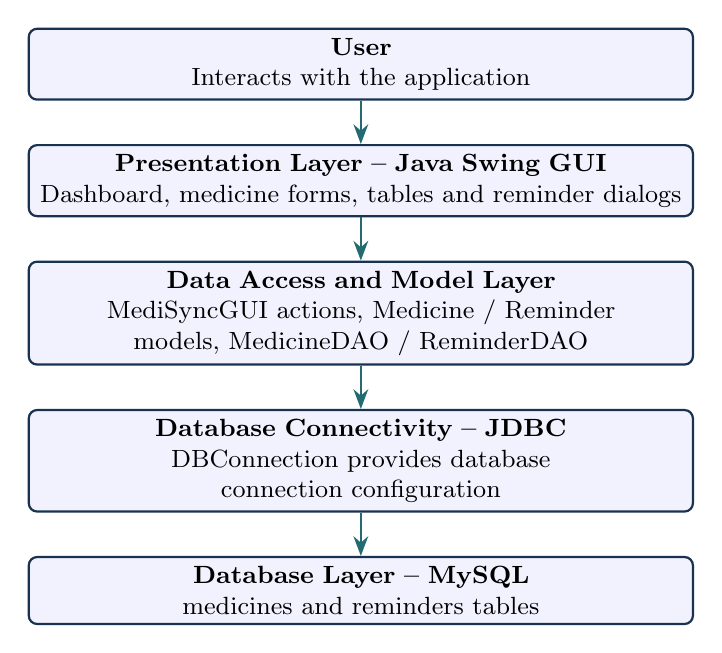
\begin{tikzpicture}[
    node distance=0.55cm,
    architecturebox/.style={
        rectangle, rounded corners=3pt, draw=MediNavy, thick,
        fill=blue!5, text width=8.2cm, minimum height=0.85cm,
        align=center, font=\small
    },
    flowarrow/.style={-{Stealth[length=2.5mm]}, thick, draw=MediTeal}
]
\node[architecturebox] (user) {\textbf{User}\\Interacts with the application};
\node[architecturebox, below=of user] (gui) {\textbf{Presentation Layer -- Java Swing GUI}\\Dashboard, medicine forms, tables and reminder dialogs};
\node[architecturebox, below=of gui] (dao) {\textbf{Data Access and Model Layer}\\MediSyncGUI actions, Medicine / Reminder models, MedicineDAO / ReminderDAO};
\node[architecturebox, below=of dao] (jdbc) {\textbf{Database Connectivity -- JDBC}\\DBConnection provides database connection configuration};
\node[architecturebox, below=of jdbc] (db) {\textbf{Database Layer -- MySQL}\\medicines and reminders tables};
\draw[flowarrow] (user) -- (gui);
\draw[flowarrow] (gui) -- (dao);
\draw[flowarrow] (dao) -- (jdbc);
\draw[flowarrow] (jdbc) -- (db);
\end{tikzpicture}
\caption{MediSync system architecture showing the interaction between the user interface, application data-access components, JDBC and MySQL.}
\label{fig:medisync-architecture}
\end{figure}

\section{Modules}
\textbf{Dashboard:} summary indicators for total medicines, low stock, expiring/expired records and active reminders. The captured dashboard shows 10, 4, 0 and 0 respectively.

\textbf{Medicine Management:} search, show, add, edit, update stock and delete actions. The table displays ID, name, type, dosage, stock, low threshold, expiry and notes.

\textbf{Stock \& Expiry:} filters for all medicines, low stock, expired and expiring within 30 days. Four records are labelled LOW STOCK in the captured view.

\textbf{Reminders:} selection of a medicine, date/time entry, scheduling and outcome recording. The supplied screenshot shows a due notification for Paracetamol.

\textbf{History:} displays reminder records. The supplied screenshot shows three TAKEN records.

\section{Database Relationship}
The \texttt{medicines.medicine\_id} column is the primary key. \texttt{reminders.medicine\_id} is a non-null foreign key referencing it with ON DELETE CASCADE. One medicine can have multiple reminders.

\section{Reminder Status Model}
The schema permits PENDING, NOTIFIED, TAKEN, MISSED and SKIPPED. PENDING represents a scheduled reminder; NOTIFIED represents a triggered notification; the final outcomes are selected by the user. A notification is not proof of consumption.

\chapter{Implementation of OOP Concepts}
The project separates domain data, database operations and user-interface responsibilities. \texttt{Medicine} and \texttt{Reminder} represent domain entities. DAO classes centralise persistence operations and abstract SQL details from the GUI. \texttt{DBConnection} abstracts connection creation. Swing itself uses framework inheritance; custom application-specific inheritance and polymorphism should be verified against the source code before being claimed.

\chapter{Implementation of Advanced Java Concepts}
\section{Swing Event Handling}
The interface responds to button clicks, tab navigation, row selection and dialog confirmation through event listeners.

\section{Timer-Based Reminder Checking}
The project context indicates that a \texttt{javax.swing.Timer} checks for due reminders at a five-second interval; Swing timer behaviour is documented in the Java API \cite{timer}. Swing timer listeners execute on the Event Dispatch Thread. Database operations in that listener should be short or moved to a background worker to avoid blocking the interface.

\section{JDBC and Maven}
JDBC connects Java to MySQL \cite{jdbc}. Parameterised statements and try-with-resources are recommended for safe SQL execution and resource cleanup \cite{preparedstatement}. Maven manages dependencies and the build through \texttt{pom.xml} \cite{maven}. The earlier build issue was an XML parsing error in the POM, not a Java compilation error.

\section{Date and Time}
Reminder scheduling depends on comparing stored DATETIME values with the application or database clock. Consistent timezone configuration is important when interpreting scheduled and notified timestamps.

\chapter{Graphical User Interface (GUI)}
The GUI uses a light workspace, dark navigation panel and teal action controls. The following figures are genuine screenshots supplied for this report.

\begin{figure}[H]\centering\includegraphics[width=\linewidth]{01_dashboard.png}\caption{Dashboard summary: 10 medicines, 4 low-stock records, 0 expiring/expired records and 0 active reminders.}\end{figure}
\begin{figure}[H]\centering\includegraphics[width=\linewidth]{02_medicine_inventory.png}\caption{Medicine inventory table showing ten medicine records.}\end{figure}
\begin{figure}[H]\centering\includegraphics[width=\linewidth]{03_stock_expiry.png}\caption{Stock and expiry alert view; four records are labelled LOW STOCK.}\end{figure}
\begin{figure}[H]\centering\includegraphics[width=\linewidth]{04_reminder_notification.png}\caption{Due-reminder notification dialog for Paracetamol.}\end{figure}
\begin{figure}[H]\centering\includegraphics[width=\linewidth]{06_reminder_history.png}\caption{Reminder history with three TAKEN outcomes.}\end{figure}

\chapter{Database Connectivity Using JDBC}
\section{Database Configuration}
The database is named \texttt{medicine\_system}, uses utf8mb4 and utf8mb4\_unicode\_ci, and is accessed using JDBC. The table definitions and constraints follow the supplied project schema and MySQL reference documentation \cite{mysql}. The project connection URL is \texttt{jdbc:mysql://localhost:3306/medicine\_system?serverTimezone=UTC}. Credentials should remain in environment variables and should not be placed in the report.

\section{Medicines Table}
The table contains medicine\_id INT primary key auto-increment, name VARCHAR(100), type VARCHAR(50), dosage VARCHAR(100), quantity INT, low\_stock\_threshold INT, expiry\_date DATE, notes VARCHAR(500), and created\_at TIMESTAMP. Quantity and threshold have non-negative checks. Indexes are defined on name and expiry\_date.

\section{Reminders Table}
The table contains reminder\_id INT primary key auto-increment, medicine\_id INT foreign key, reminder\_time DATETIME, status VARCHAR(20), notified\_at nullable DATETIME, completed\_at nullable DATETIME, and created\_at TIMESTAMP. A check constraint restricts the status values. An index on (status, reminder\_time) supports due-reminder lookup.

\begin{figure}[H]\centering\includegraphics[width=0.9\linewidth]{07_sql_reminders.png}\caption{MySQL Workbench result grid for reminder records.}\end{figure}
\begin{figure}[H]\centering\includegraphics[width=0.9\linewidth]{08_sql_medicines.png}\caption{MySQL Workbench result grid for medicine records.}\end{figure}

\chapter{Source Code and Output Screenshots}
The main source components are \texttt{MediSyncGUI.java}, \texttt{Medicine.java}, \texttt{Reminder.java}, \texttt{MedicineDAO.java}, \texttt{ReminderDAO.java} and \texttt{DBConnection.java}. The \texttt{pom.xml} file defines Maven build configuration and dependencies.

The schema creation script should contain database and table definitions. Diagnostic queries such as \texttt{SELECT * FROM medicines} and \texttt{SELECT * FROM reminders} are better kept in a separate database testing script.

\textbf{Build:} \texttt{mvn clean compile}\\
\textbf{Run:} \texttt{mvn exec:java "-Dexec.mainClass=gui.MediSyncGUI"}

\chapter{Testing and Results}
The results below are limited to the supplied application and MySQL screenshots. They are reported as observed evidence rather than as a claim that every possible test case has been executed.

\begin{table}[H]
\centering
\small
\begin{tabularx}{\textwidth}{>{\raggedright\arraybackslash}p{0.28\textwidth} X >{\raggedright\arraybackslash}p{0.20\textwidth}}
\toprule
\textbf{Test case} & \textbf{Expected behaviour} & \textbf{Evidence status} \\
\midrule
Dashboard summary & Display inventory and reminder summary counts. & Observed: 10 medicines, 4 low-stock, 0 expiring/expired, 0 active reminders. \\
Medicine inventory & Display stored medicine records and inventory fields. & Observed: 10 records displayed. \\
Low-stock monitoring & Identify records where quantity is below the configured threshold. & Observed: 4 records labelled LOW STOCK. \\
Expiry monitoring & Provide filters for expired and expiring records. & Interface observed; no matching expiry alert shown in supplied capture. \\
Reminder notification & Display a notification when a reminder becomes due. & Observed: Paracetamol notification popup. \\
Reminder history & Display reminder records and recorded outcomes. & Observed: 3 records with TAKEN status. \\
MySQL persistence & Retain medicine and reminder records in database tables. & Observed in MySQL Workbench result grids. \\
MISSED / SKIPPED outcomes & Allow user to record these outcomes. & Not demonstrated in supplied screenshots. \\
Database failure handling & Present controlled feedback when database access fails. & Not demonstrated in supplied screenshots. \\
Input validation and delete cascade & Reject invalid data and maintain referential integrity. & Not demonstrated by supplied screenshots. \\
\bottomrule
\end{tabularx}
\caption{Evidence-based functional test summary.}
\end{table}

The dashboard shows 10 medicines, 4 low-stock records, 0 expiring/expired records and 0 active reminders at capture time. The inventory view displays ten medicine records. The stock view marks four records LOW STOCK. A Paracetamol due-reminder notification was captured. Reminder history shows three records, all TAKEN. MySQL Workbench result grids show medicine and reminder rows.

MISSED and SKIPPED outcomes, database failure handling, invalid input handling and delete-cascade behaviour are not demonstrated in the supplied screenshots and are not claimed as tested. One reminder row in the SQL screenshot has a NULL \texttt{notified\_at}; therefore, the report does not assume all reminder rows followed an identical notification path.

\chapter{Conclusion and Future Enhancements}
MediSync demonstrates integration of Java Swing, object-oriented program organisation, JDBC and MySQL in a desktop application for medicine inventory and reminder management. The evidence shows inventory records, low-stock alerts, a due reminder notification, reminder history and corresponding SQL records.

Future enhancements include background scheduling off the Swing Event Dispatch Thread, recurring reminders, MISSED/SKIPPED reporting, authentication, database backup and restore, CSV/PDF export, stronger validation, operating-system notifications and automated unit/integration tests. The application is an inventory and reminder aid, not a substitute for medical advice.

\appendix
\chapter{Reminder Workflow}
Figure~\ref{fig:medisync-reminder-workflow} illustrates the reminder lifecycle implemented by the application. The flow represents the reminder process while the desktop application is running.

\begin{figure}[H]
\centering
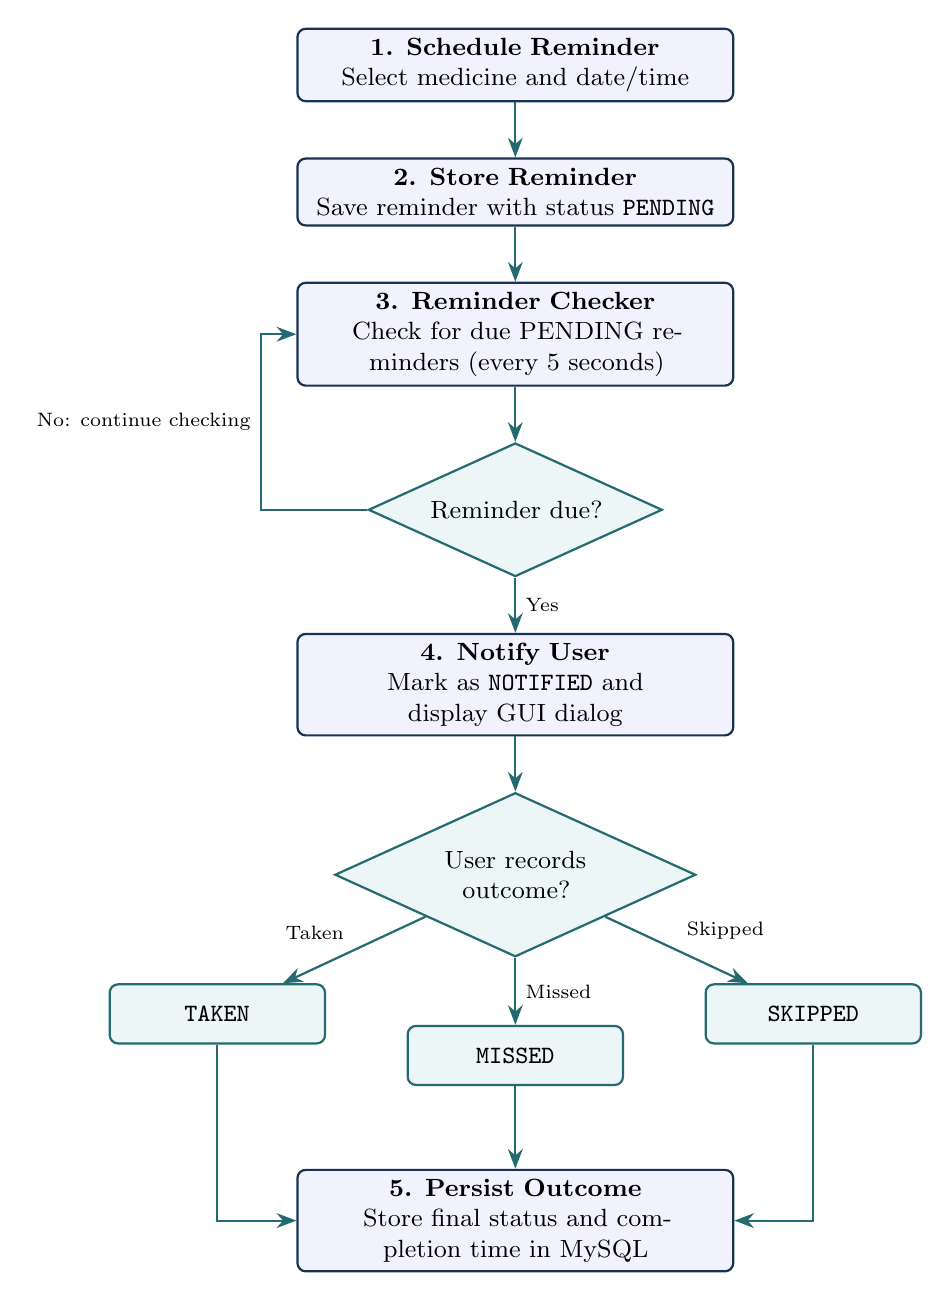
\begin{tikzpicture}[
    node distance=0.7cm and 0.9cm,
    process/.style={
        rectangle, rounded corners=3pt, draw=MediNavy, thick,
        fill=blue!5, text width=5.3cm, minimum height=0.85cm,
        align=center, font=\small
    },
    decision/.style={
        diamond, aspect=2.2, draw=MediTeal, thick, fill=teal!7,
        text width=2.8cm, align=center, inner sep=2pt, font=\small
    },
    outcome/.style={
        rectangle, rounded corners=3pt, draw=MediTeal, thick,
        fill=teal!7, text width=2.5cm, minimum height=0.75cm,
        align=center, font=\small
    },
    flowarrow/.style={-{Stealth[length=2.5mm]}, thick, draw=MediTeal}
]
\node[process] (schedule) {\textbf{1. Schedule Reminder}\\Select medicine and date/time};
\node[process, below=of schedule] (pending) {\textbf{2. Store Reminder}\\Save reminder with status \texttt{PENDING}};
\node[process, below=of pending] (checker) {\textbf{3. Reminder Checker}\\Check for due PENDING reminders (every 5 seconds)};
\node[decision, below=of checker] (due) {Reminder due?};
\node[process, below=of due] (notify) {\textbf{4. Notify User}\\Mark as \texttt{NOTIFIED} and display GUI dialog};
\node[decision, below=of notify] (response) {User records outcome?};
\node[outcome, below left=0.85cm and 1.25cm of response] (taken) {\textbf{\texttt{TAKEN}}};
\node[outcome, below=0.85cm of response] (missed) {\textbf{\texttt{MISSED}}};
\node[outcome, below right=0.85cm and 1.25cm of response] (skipped) {\textbf{\texttt{SKIPPED}}};
\node[process, below=1.05cm of missed] (save) {\textbf{5. Persist Outcome}\\Store final status and completion time in MySQL};

\draw[flowarrow] (schedule) -- (pending);
\draw[flowarrow] (pending) -- (checker);
\draw[flowarrow] (checker) -- (due);
\draw[flowarrow] (due) -- node[right, font=\scriptsize]{Yes} (notify);
\draw[flowarrow] (due.west) -- ++(-1.35,0) |- node[pos=0.25, left, font=\scriptsize]{No: continue checking} (checker.west);
\draw[flowarrow] (notify) -- (response);
\draw[flowarrow] (response) -- node[above left, font=\scriptsize]{Taken} (taken);
\draw[flowarrow] (response) -- node[right, font=\scriptsize]{Missed} (missed);
\draw[flowarrow] (response) -- node[above right, font=\scriptsize]{Skipped} (skipped);
\draw[flowarrow] (taken) |- (save);
\draw[flowarrow] (missed) -- (save);
\draw[flowarrow] (skipped) |- (save);
\end{tikzpicture}
\caption{MediSync reminder workflow from scheduling through notification and user-recorded outcome.}
\label{fig:medisync-reminder-workflow}
\end{figure}

\begin{enumerate}
\item The user selects a medicine and schedules a date/time; the record is inserted as PENDING.
\item While the application is running, the reminder checker looks for due PENDING reminders.
\item A due reminder can be marked NOTIFIED and \texttt{notified\_at} can record the notification time; the GUI displays a dialog.
\item The user records TAKEN, MISSED or SKIPPED; the outcome and \texttt{completed\_at} are stored.
\end{enumerate}
The screenshots demonstrate a notification and TAKEN outcomes. MISSED and SKIPPED are allowed by the schema but are not shown in the supplied screenshots.

\chapter{Demonstration Sequence}
\begin{enumerate}
\item Launch the application after confirming MySQL is running.
\item Explain the Dashboard summary.
\item Show the Medicines table and record actions.
\item Demonstrate Stock \& Expiry filters.
\item Schedule a near-future reminder.
\item Wait for the notification while the application remains open.
\item Record an outcome and verify it in History.
\item Run SELECT queries in MySQL Workbench to show persisted records.
\end{enumerate}


\begin{thebibliography}{9}

\bibitem{java}
Oracle,
\textit{Java Platform, Standard Edition Documentation}.
Available at: \url{https://docs.oracle.com/en/java/}

\bibitem{swing}
Oracle,
\textit{Creating a GUI With Swing}.
Available at: \url{https://docs.oracle.com/javase/tutorial/uiswing/}

\bibitem{jdbc}
Oracle,
\textit{JDBC Database Access}.
Available at: \url{https://docs.oracle.com/javase/tutorial/jdbc/}

\bibitem{timer}
Oracle,
\textit{Java SE API Documentation: javax.swing.Timer}.
Available at: \url{https://docs.oracle.com/en/java/javase/17/docs/api/java.desktop/javax/swing/Timer.html}

\bibitem{preparedstatement}
Oracle,
\textit{Java SE API Documentation: PreparedStatement}.
Available at: \url{https://docs.oracle.com/en/java/javase/17/docs/api/java.sql/java/sql/PreparedStatement.html}

\bibitem{mysql}
MySQL,
\textit{MySQL 8.0 Reference Manual}.
Available at: \url{https://dev.mysql.com/doc/refman/8.0/en/}

\bibitem{connector}
MySQL,
\textit{MySQL Connector/J Developer Guide}.
Available at: \url{https://dev.mysql.com/doc/connector-j/en/}

\bibitem{maven}
Apache Software Foundation,
\textit{Apache Maven Documentation}.
Available at: \url{https://maven.apache.org/guides/}

\bibitem{project}
MediSync Project Team,
\textit{MediSync: Medicine Reminder and Stock Monitoring System}.
Project source code, database schema, and implementation screenshots.
SRM University--AP, 2026.

\end{thebibliography}
\end{document}
